\documentclass[12pt,a4paper]{article}
\usepackage[polish]{babel}
\usepackage[T1]{fontenc}
\usepackage{hyperref}
\usepackage{url}
\usepackage{graphicx}
\graphicspath{ {images/} }
\usepackage{csquotes}
\usepackage[utf8x]{inputenc}
\usepackage{fancyvrb}

\addtolength{\hoffset}{-1.5cm}
\addtolength{\marginparwidth}{-1.5cm}
\addtolength{\textwidth}{3cm}
\addtolength{\voffset}{-1cm}
\addtolength{\textheight}{2.5cm}
\setlength{\topmargin}{0cm}
\usepackage{algorithm}
\usepackage[noend]{algpseudocode}
\setlength{\headheight}{0cm}

\begin{document}
    \begin{titlepage}
       \begin{center}
           \vspace*{1cm}
           
           {\fontsize{23}{25}\selectfont Dokumentacja projektu\\Programowanie obiektowe i graficzne}
     
            \vspace{1.0cm}
        
            {\fontsize{17}{18}\selectfont Dawid Bitner \\ Marcin Krupa}
           
            \vspace{0.4cm}
           
            {\fontsize{12}{13}\selectfont 1 lipca 2019}
           
            \vfill
            \vspace{0.8cm}
     
            {\fontsize{13}{14}\selectfont Politechnika Śląska\\Wydział Matematyki Stosowanej\\Rok akademicki 2018/2019}
     
       \end{center}
    \end{titlepage}
	\newpage
	\tableofcontents
	\newpage
	\section{Część I}
	\subsection{Opis projektu}
        Postanowiliśmy stworzyć na projekt z przedmiotu \textit{Programowanie obiektowe i graficzne} aplikację użytkową obsługującą nasz projekt stworzony na przedmiot \textit{Bazy danych}. Aplikacja umożliwia wyszukiwanie danych w bazie dotyczącej piłkarskiej ekstraklasy, ich dodawanie i edytowanie, zależnie od typu konta jakim zaloguje się użytkownik.
        
    \subsection{Założenia projektowe}
    -Utworzenie dwóch typów kont: administrator i  użytkownik. \\
    -Umożliwienie im logowania do aplikacji, dostępu do danych w bazie według typu konta. \\
    -Każde z kont ma inne możliwości:\\
    a)Konto użytkownika pozwala tylko na wyświetlanie danych znajdujących się w bazie według określonych reguł\\
    b)Konto administratora pozwala na wyświetlanie, edycję i dodawanie danych znajdujących się w bazie \\
    -Do edytowania/przeglądania dostępne są tabele: kluby, gracze, puchar krajowy, stadiony etc \\
    -Informacje o klubie: pokazuje aktualnych zawodników i trenera, herb, nazwę, stadion etc \\
    -Szczegółowe informacje o wybranych zawodnikach. \\
    -Dodawanie danych do bazy (administrator). \\
    -Możliwość przełączania pomiędzy zakładkami. \\
    -Zabezpieczenia przed sql injection. \\
    -Model MVP. \\
    -Projekt wzorowany jest na aplikacji EXTRANET PZPN. \\
    
    \newpage
    \section{Część II}
    \subsection{Instrukcja użytkowania}
    Program został stworzony z myślą o wykorzystaniu go przez użytkowników dwóch typów kont: administratora oraz zwykłego użytkownika. Każdy z tych typów kont zapewnia inną funkcjonalność, która została odzwierciedlona w programie.
    
    Aby prawidłowo korzystać z funkcjonalności programu, należy mieć połączenie z Internetem. Po uruchomieniu programu z pliku $application.exe$ użytkownikowi pojawi się ekran logowania.
    
    \begin{center}
        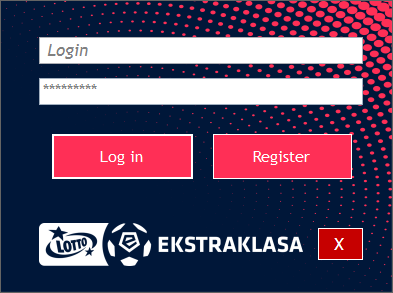
\includegraphics[scale=1]{login-panel.png}
        \begin{flushleft}
            \begin{scriptsize}
            \begin{list}{}{\leftmargin=21.5em}\raggedright\item\relax
            Rysunek 1: Ekran logowania.
            \end{list}
            \end{scriptsize}
        \end{flushleft}
    \end{center}
    
    Użytkownik, według założeń projektu, ma możliwość wyłącznie przeglądania rekordów w bazie. Administrator natomiast posiada niemal pełną kontrolę nad bazą. W zależności od tego na jaki typ konta zaloguje się użytkownik, pojawi mu się inna forma z programem, różniąca się przede kontrolką umożliwiającą przełączanie się pomiędzy panelami.
    
    \begin{center}
        
\includegraphics[scale=1]{admin-controls.png}
        \begin{flushleft}
            \begin{scriptsize}
            \begin{list}{}{\leftmargin=19em}\raggedright\item\relax
            Rysunek 2: Kontrolka administratora.
            \end{list}
            \end{scriptsize}
        \end{flushleft}
    \end{center}
    
    Kontrolki kolejno od lewej do prawej oznaczają:
    \begin{itemize}
        \item wybór panelu wyszukiwania,
        \item wybór panelu wprowadzania rekordów do tabeli,
        \item wybór panelu usuwania rekordu z tabeli,
        \item wybór panelu aktualizacji rekordu w tabeli.
    \end{itemize}
    
    \subsubsection{Panel wyszukiwania}
    Panel ten jest dostępny zarówno dla administratora jak i użytkownika.
    \begin{center}
        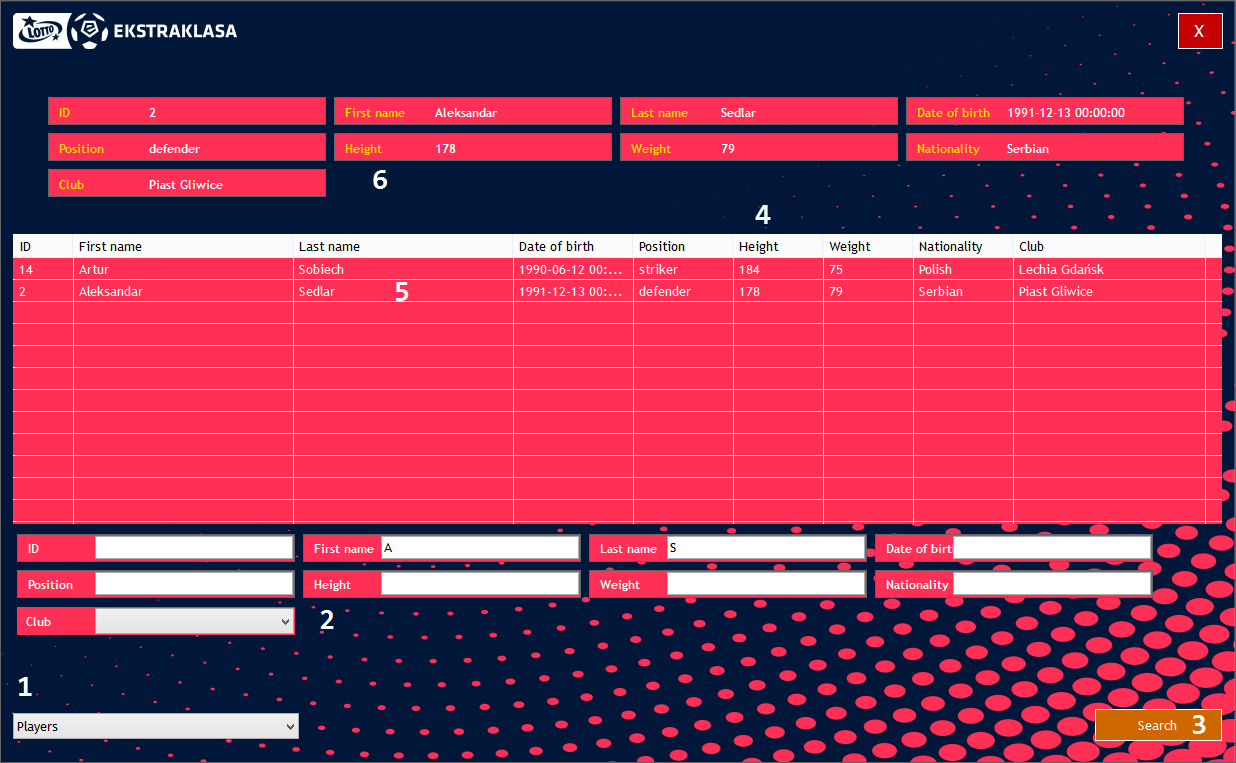
\includegraphics[scale=0.47]{select-panel.png}
        \begin{flushleft}
            \begin{scriptsize}
            \begin{list}{}{\leftmargin=13.5em}\raggedright\item\relax
            Rysunek 3: Panel wyszukiwania z przykładowym wynikiem zapytania.
            \end{list}
            \end{scriptsize}
        \end{flushleft}
    \end{center}
    
    Aby wyszukiwać rekordy w bazie:
    \begin{enumerate}
        \item Należy wybrać tabele z której chcemy wyszukiwać nasze rekordy z rozwijanej listy z tabelami.
        \item Następnie określamy kryteria zapytań. Krok ten można pominąć jeśli chcemy wyświetlić wszystkie rekordy w tabeli.
        \item Naciskając przycisk $Search$ wyszukujemy rekordy w bazie. Jeśli użytkownik nie określił tabeli z której chce wyszukiwać rekordy, nic się nie wydarzy.
        \item Wyświetlone rekordy można sortować. W tym celu należy kliknąć w nazwę kolumny (na powyższym przykładzie pokazano sortowanie po kolumnie $Height$).
        \item Naciskając dwukrotnie w rekord wyświetlą nam się nad tabelą dane dotyczące konkretnego elementu.
        \item Dane dotyczące rekordu wskazanego dwuklikiem.
    \end{enumerate}
    
    \newpage
    
    \subsubsection{Panel wprowadzania rekordów do tabeli}
    Dostępny tylko dla administratora, umożliwia wprowadzanie rekordów do wybranej tabeli.
    \begin{center}
        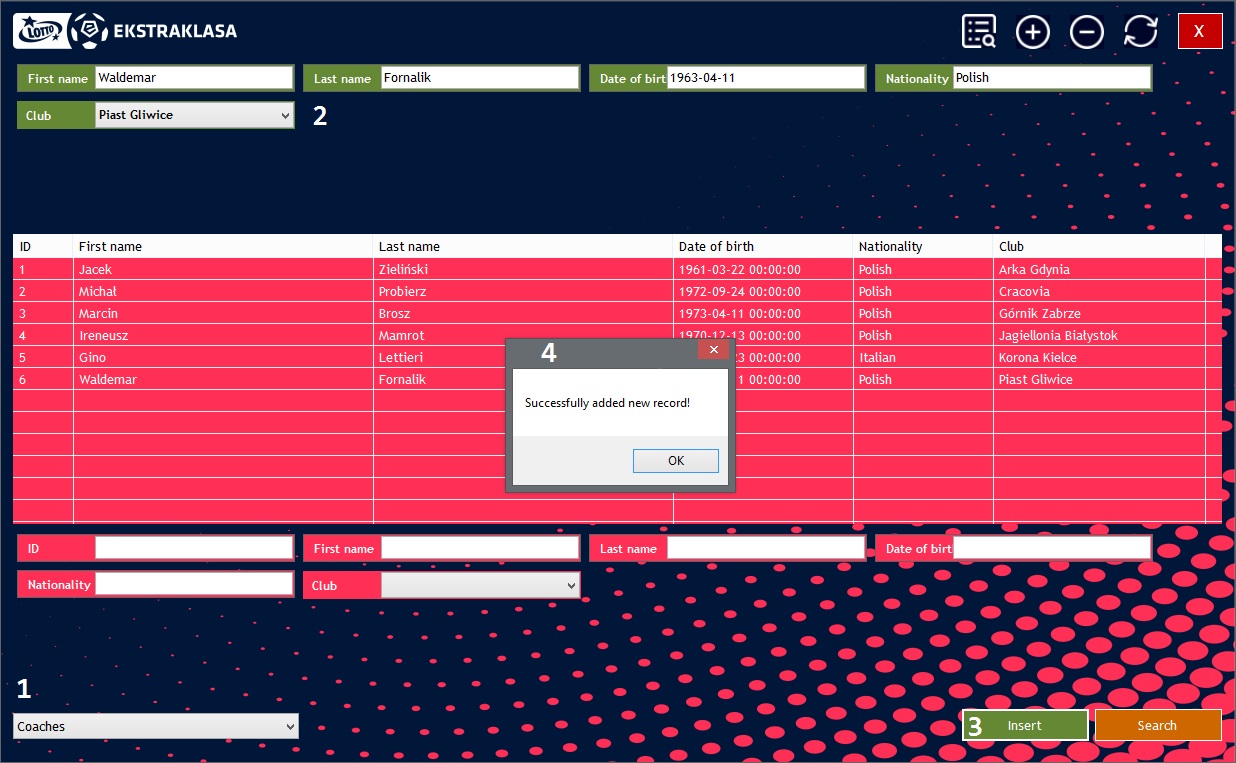
\includegraphics[scale=0.47]{insert-panel.png}
        \begin{flushleft}
            \begin{scriptsize}
            \begin{list}{}{\leftmargin=13.5em}\raggedright\item\relax
            Rysunek 4: Panel wprowadzania rekordów do tabeli, z przykładowym trenerem.
            \end{list}
            \end{scriptsize}
        \end{flushleft}
    \end{center}
    
    Aby wprowadzać rekordy do tabeli:
    \begin{enumerate}
        \item Należy wybrać tabele do której chcemy wprowadzać nowe rekordy z rozwijalnej listy.
        \item Ukażą się nam u góry kontrolki z miejscem na wpisanie nowego rekordu w tabeli. Dla ułatwienia w dalszym ciągu można wyszukiwać rekordy w tabeli.
        \item Naciskając przycisk $Insert$ zatwierdzamy wprowadzenie rekordu do tabeli. Ważnym jest, aby były wprowadzone wszystkie dane. W innym przypadku użytkownik zostanie powiadomiony o ich braku.
        \item Po akcji wprowadzenia rekordu do tabeli, użytkownik zostaje powiadomiony o udanej lub nieudanej próbie wprowadzenia rekordu do tabeli.
    \end{enumerate}
    
    \newpage
    
    \subsubsection{Panel usuwania rekordu w tabeli}
    Dostępny tylko dla administratora, umożliwia usuwanie pojedynczego rekordu z tabeli.
    \begin{center}
        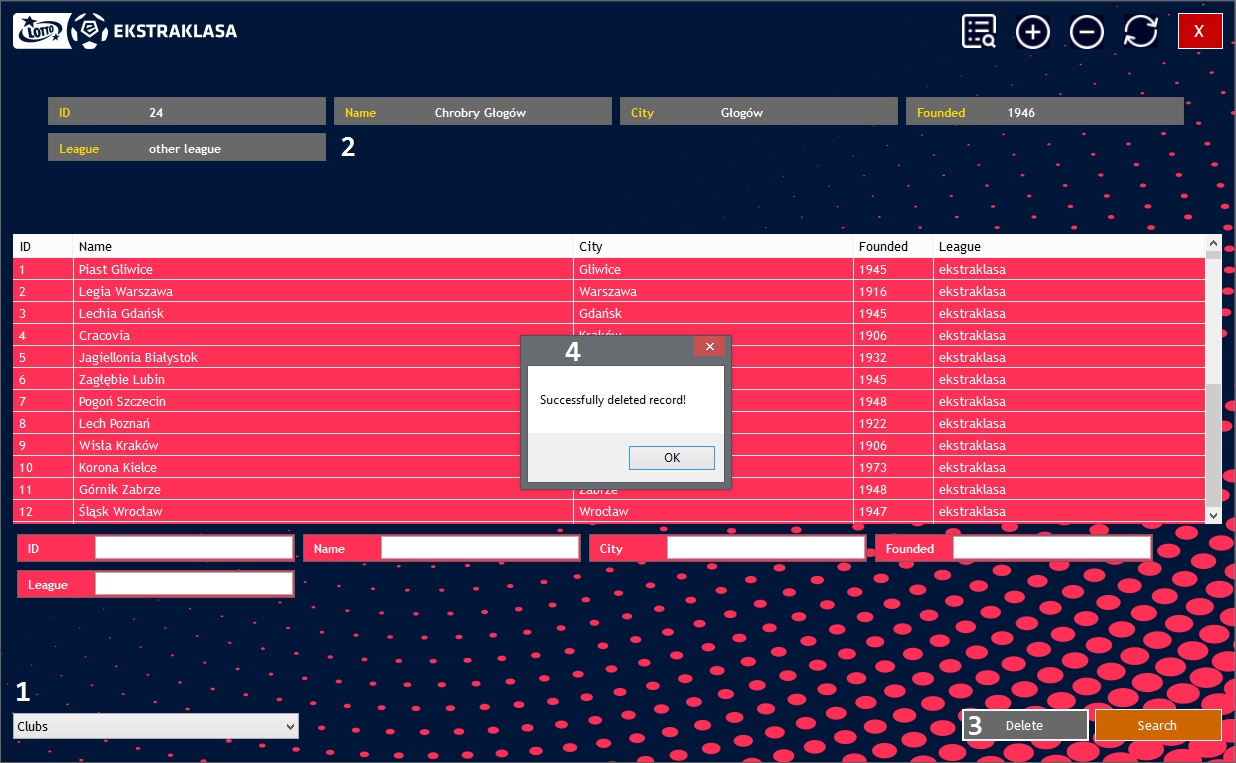
\includegraphics[scale=0.47]{delete-panel.png}
        \begin{flushleft}
            \begin{scriptsize}
            \begin{list}{}{\leftmargin=13.5em}\raggedright\item\relax
            Rysunek 5: Panel usuwania rekordu z tabeli, z przykładowym klubem.
            \end{list}
            \end{scriptsize}
        \end{flushleft}
    \end{center}
    
    Aby usuwać rekordy z tabeli:
    \begin{enumerate}
        \item Należy wybrać tabele z której chcemy usunąć wybrany rekord z rozwijalnej listy.
        \item Naciskając dwukrotnie w rekord wyświetlą nam się nad tabelą dane dotyczące tego rekordu. Dopiero wykonując te czynność określamy jaki element chcemy usunąć z tabeli.
        \item Naciskając przycisk $Delete$ zatwierdzamy usunięcie rekordu z tabeli.
        \item Po akcji usunięcia rekordu z tabeli, użytkownik zostaje powiadomiony o udanej lub nieudanej próbie usunięcia rekordu z tabeli.
    \end{enumerate}
    
    \newpage
    
    \subsubsection{Panel edytowania rekordu w tabeli}
    Dostępny tylko dla administratora, umożliwia edytowanie pojedynczego rekordu z tabeli.
    \begin{center}
        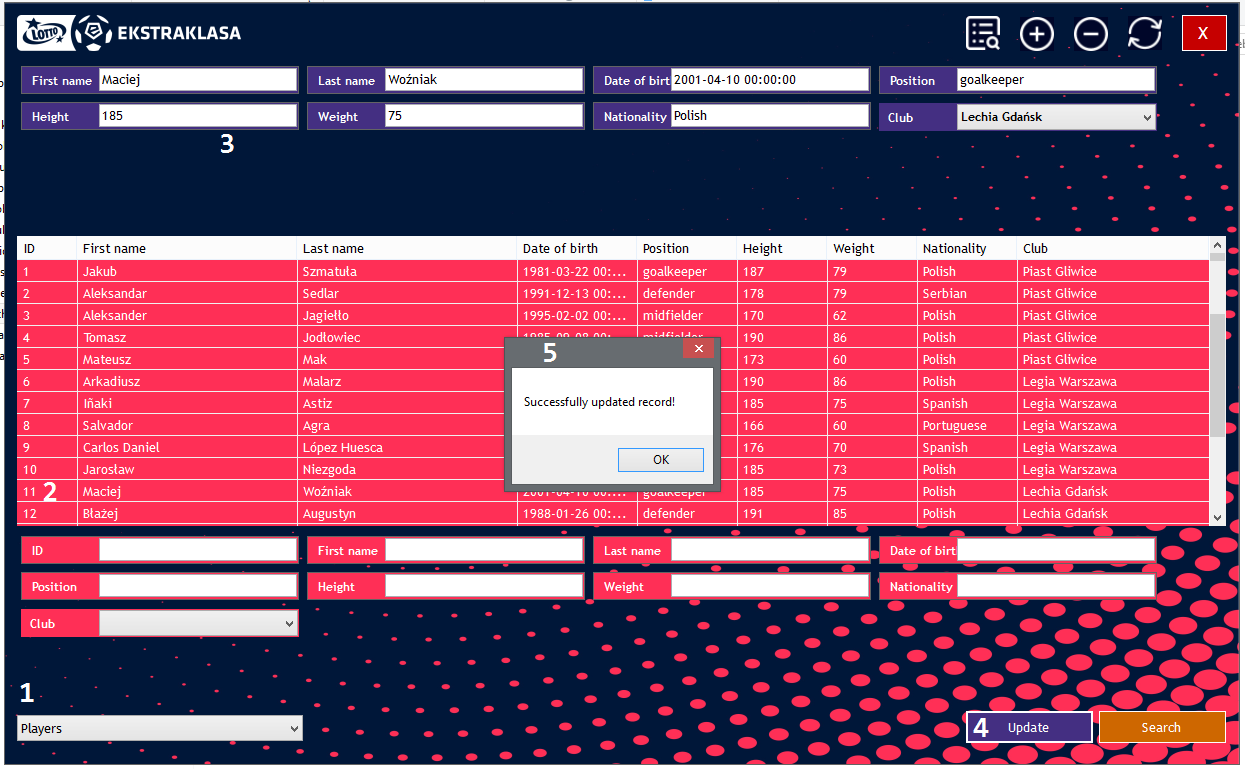
\includegraphics[scale=0.47]{update-panel.png}
        \begin{flushleft}
            \begin{scriptsize}
            \begin{list}{}{\leftmargin=13.5em}\raggedright\item\relax
            Rysunek 6: Panel edytowania rekordu w tabeli, z przykładowym graczem.
            \end{list}
            \end{scriptsize}
        \end{flushleft}
    \end{center}
    
    Aby usuwać rekordy z tabeli:
    \begin{enumerate}
        \item Należy wybrać tabele w której chcemy edytować wybrany rekord z rozwijalnej listy.
        \item Naciskając dwukrotnie w rekord wyświetlą nam się nad tabelą dane dotyczące tego rekordu. Dopiero wykonując te czynność określamy jaki element chcemy edytować w tabeli.
        \item Edytujemy dane rekordu z tabeli. 
        \item Naciskając przycisk $Update$ zatwierdzamy edycje rekordu z tabeli. Ważnym jest, aby były wprowadzone wszystkie dane. W innym przypadku użytkownik zostanie powiadomiony o ich braku.
        \item Po akcji edytowania rekordu w tabeli, użytkownik zostaje powiadomiony o udanej lub nieudanej próbie edytowania rekordu w tabeli.
    \end{enumerate}
    
    \newpage

    \section{Część III}
    \subsection{Implementacja}
    Środowisko programistyczne: Visual Studio 2017 \\
    Użyty framework: .NET Framework \\
    API: Windows Forms \\
    Wzorzec projektowy: MVP \\
    System kontroli wersji: Git \\
    
    \subsection{Struktura projektowa}
    Projekt został podzielony na pliki, które znajdują się w poszczególnych folderach - by zachować przejrzystość i łatwość w poruszaniu się po plikach projektowych.
    \begin{center}
        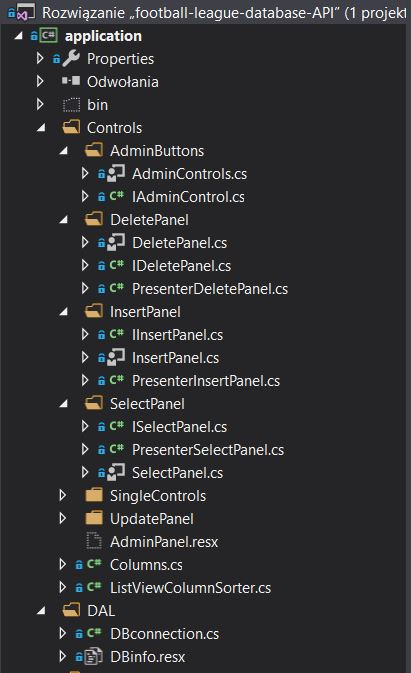
\includegraphics[scale=1]{struct.JPG} \\
        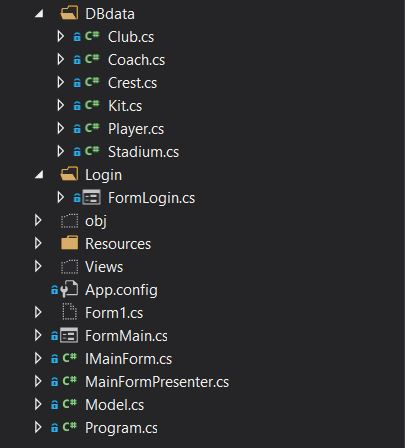
\includegraphics[scale=1]{struct2.JPG}
    \end{center}
    
    Przykładowa encja gracza:
    \begin{verbatim}
using System;
using System.Collections.Generic;
using System.Linq;
using System.Text;
using System.Threading.Tasks;
using System.Data;
using System.Globalization;

namespace application.DBdata
{
    class Player
    {
        public int Id { get; set; } // zabezpieczenie przed nullem
        public string FirstName { get; set; }
        public string LastName { get; set; }
        public DateTime BirthDate { get; set; }
        public string Position { get; set; }
        public int Height { get; set; } // 0 to 255
        public int Weight { get; set; }
        public string Nationality { get; set; }
        public string ClubPlayer { get; set; }

        public Player() { }

        public Player(int Id, string FirstName, string LastName, DateTime BirthDate,
        string Position, int Height, int Weight, string Nationality, string ClubPlayer)
        {
            this.Id = Id;
            this.FirstName = FirstName;
            this.LastName = LastName;
            this.BirthDate = DateTime.Parse(BirthDate.ToString("yyyy-MM-dd"));
            this.Position = Position;
            this.Height = Height;
            this.Weight = Weight;
            this.Nationality = Nationality;
            this.ClubPlayer = ClubPlayer;

        }
    }
}
    \end{verbatim}{}
    
    \section{Część IV}
    \subsection{Podsumowanie}
        Podsumowując, udało nam się wykonać wszystkie postawione sobie założenia dotyczące tego projektu, zadbaliśmy o przejrzystość kodu jak i czytelną szatę graficzną. Z powodzeniem wdrożyliśmy wzorzec projektowy MVP. Program jest intuicyjny i łatwy w obsłudze.
    

\end{document}
